% -*- ispell-dictionary:"american" -*-
%
% The following \documentclass options may be useful:
%
% preprint      Remove this option only once the paper is in final form.
% 10pt          To set in 10-point type instead of 9-point.
% 11pt          To set in 11-point type instead of 9-point.
% authoryear    To obtain author/year citation style instead of numeric.
\documentclass[preprint,nonatbib,10pt,nocopyrightspace]{sigplanconf}

%%%%%%%%%%%%%%%%%%%%%%%%%
%% Document and Layout %%
%%%%%%%%%%%%%%%%%%%%%%%%%

% Fix for multiple "No room for a new \dimen" errors.
%
% See: http://tex.stackexchange.com/questions/38607/no-room-for-a-new-dimen
%
\usepackage{etex}

\usepackage[utf8]{inputenc}

% Fix for "'babel/polyglossia' detected but 'csquotes' missing"
% warning. NOTE: Include after inputenc.
%
\usepackage{csquotes}

\usepackage{booktabs}

% Required for full page-width tables.
\usepackage{tabularx}

% Define column types L, C, R with known text justification and fixed
% widths:
\usepackage{array}
\newcolumntype{L}[1]{>{\raggedright\let\newline\\\arraybackslash\hspace{0pt}}m{#1}}
\newcolumntype{C}[1]{>{\centering\let\newline\\\arraybackslash\hspace{0pt}}m{#1}}
\newcolumntype{R}[1]{>{\raggedleft\let\newline\\\arraybackslash\hspace{0pt}}m{#1}}

% Make internal macro definitions accessible,
% e.g. \@title, \@date \@author.
\makeatletter

% Uncomment the following line to remove column separation:
%
%\setlength{\columnsep}{5mm}

\usepackage{color}
\newcommand{\fix}[1]{\textcolor{red}{\em\footnotesize#1}}


%%%%%%%%%%%%%%%%
% Bibliography %
%%%%%%%%%%%%%%%%
\usepackage[%
    backend=biber,
    style=numeric-comp,
    % style=numeric-comp,  % numerical-compressed
    sorting=none,        % nty,nyt,nyvt,anyt,anyvt,ynt,ydnt,none
    sortcites=true,      % sort \cite{b a d c}: true,false
    block=none,          % space between blocks: none,space,par,nbpar,ragged
    indexing=false,      % indexing options: true,false,cite,bib
    citereset=none,      % don't reset cites
    isbn=false,          % print ISBN?
    url=true,            % print URL?
    doi=false,           % print DOI?
    natbib=true,         % natbib compatability
    maxbibnames=99       % no 'et-al' in the bibliography pls
  ]{biblatex}

% My system-wide bibtex file:
\addbibresource{../../../library.bib}

% Reduce the font size of the bibliography:
\renewcommand{\bibfont}{\normalfont\scriptsize}

% No italics in \paragraph{title} style:
\usepackage{titlesec}
\titleformat*{\paragraph}{\bfseries}


%%%%%%%%%%%%%%%%%%%%%%%%%%%%%%%%%%%%%
%% Figures, footnotes and listings %%
%%%%%%%%%%%%%%%%%%%%%%%%%%%%%%%%%%%%%

\usepackage[perpage]{footmisc}

% Pre-requisites for rendering upquotes in listings package.
\usepackage[T1]{fontenc}
\usepackage{lmodern}
\usepackage{textcomp}

% Source code listings.
\usepackage{listings}
\lstset{%
  basicstyle=\scriptsize,%
  numbers=left,%
  % numberblanklines=false,
  escapeinside=||,
  frame=tb,%
  breaklines=true,%
  postbreak=\raisebox{0ex}[0ex][0ex]{\ensuremath{\color{red}\hookrightarrow\space}},% red arrow at line breaks
  captionpos=b%
}

\let\origthelstnumber\thelstnumber
\newcommand*\Suppressnumber{%
  \lst@AddToHook{OnNewLine}{%
    \let\thelstnumber\relax%
     \advance\c@lstnumber-\@ne\relax%
    }%
}

\newcommand*\Reactivatenumber{%
  \lst@AddToHook{OnNewLine}{%
   \let\thelstnumber\origthelstnumber%
   \advance\c@lstnumber\@ne\relax}%
}

% OpenCL listings
%
% From: http://gpumodeling.blogspot.com/2011/06/opencl-programs-in-latex-listings.html
 \lstdefinelanguage[OpenCL]{C}[ANSI]{C}
{morekeywords={__kernel,kernel,__local,local,__global,global,%
__constant,constant,__private,private,%
char2,char3,char4,char8,char16,%
uchar2,uchar3,uchar4,uchar8,uchar16,%
short2,short3,short4,short8,short16,%
ushort2,ushort3,ushort4,ushort8,ushort16,%
int2,int3,int4,int8,int16,%
uint2,uint3,uint4,uint8,uint16,%
long2,long3,long4,long8,long16,%
ulong2,ulong3,ulong4,ulong8,ulong16,%
float2,float3,float4,float8,float16,%
image2d_t,image3d_t,sampler_t,event_t,%
bool2,bool3,bool4,bool8,bool16,%
half2,half3,half4,half8,half16,%
quad,quad2,quad3,quad4,quad8,quad16,%
complex,imaginary},%
}%

% Pseudo-code listings.
\usepackage{algorithm}
\usepackage{algpseudocode}
\newcommand{\Break}{\State \textbf{break} }
\algblockdefx[Loop]{Loop}{EndLoop}[1][]{\textbf{Loop} #1}{\textbf{End
    Loop}}

\algrenewcommand\ALG@beginalgorithmic{\footnotesize}

%%%%%%%%%%%%%%%%%%%%%%%%
%% Graphics and maths %%
%%%%%%%%%%%%%%%%%%%%%%%%
\usepackage{amsmath}

% Plots:
\usepackage{filecontents}
\usepackage{pgfplots, pgfplotstable}
\usepgfplotslibrary{statistics}

\usepackage{tikz}

% Tikz flowchart configuration.
\usetikzlibrary{shapes,arrows,shadows,fit,backgrounds}
\tikzstyle{decision} = [diamond,
                        draw,
                        text width=4.5em,
                        text badly centered,
                        node distance=3cm,
                        inner sep=0pt]
\tikzstyle{block}    = [rectangle,
                        draw,
                        text width=5em,
                        text centered,
                        node distance=3cm,
                        minimum height=4em,
                        inner sep=.2cm]
\tikzstyle{line}     = [draw, -latex']

% Smaller font:
\pgfplotsset{every tick label/.append style={font=\scriptsize}}

% Vector notation, e.g. \vv{x}:
%
\usepackage{esvect}

% Additional amsmath symbols, see:
%
% http://texblog.org/2007/08/27/number-sets-prime-natural-integer-rational-real-and-complex-in-latex/
%
\usepackage{amsfonts}
\usepackage{amssymb}

\usepackage{graphicx}
\usepackage{mathtools}

% Provide bold font face in maths.
\usepackage{bm}

% Use either 'subfig' or 'subcaption', NOT BOTH!
\usepackage{subfig}
% \usepackage{subcaption}
% \expandafter\def\csname ver@subfig.sty\endcsname{}

% Define an 'myalignat' command which behave as 'alignat' without the
% vertical top and bottom padding. See:
%     http://www.latex-community.org/forum/viewtopic.php?f=5&t=1890
\newenvironment{myalignat}[1]{%
  \setlength{\abovedisplayskip}{-.7\baselineskip}%
  \setlength{\abovedisplayshortskip}{\abovedisplayskip}%
  \start@align\z@\st@rredtrue#1
}%
{\endalign}

% Define additional operators:
\DeclareMathOperator*{\argmin}{arg\,min}
\DeclareMathOperator*{\argmax}{arg\,max}

\DeclareMathOperator*{\gain}{Gain}

% Skeleton operators.
\DeclareMathOperator*{\map}{Map}
\DeclareMathOperator*{\reduce}{Reduce}
\DeclareMathOperator*{\scan}{Scan}
\DeclareMathOperator*{\stencil}{Stencil}
\DeclareMathOperator*{\zip}{Zip}
\DeclareMathOperator*{\allpairs}{All\,Pairs}

% Define a command to allow word breaking.
\newcommand*\wrapletters[1]{\wr@pletters#1\@nil}
\def\wr@pletters#1#2\@nil{#1\allowbreak\if&#2&\else\wr@pletters#2\@nil\fi}

% Define a command to create centred page titles.
\newcommand{\centredtitle}[1]{
  \begin{center}
    \large
    \vspace{0.9cm}
    \textbf{#1}
  \end{center}}

% Provide generic commands \degree, \celsius, \perthousand, \micro
% and \ohm which work both in text and maths mode.
\usepackage{gensymb}

\begin{document}

\special{papersize=8.5in,11in}
\setlength{\pdfpageheight}{\paperheight}
\setlength{\pdfpagewidth}{\paperwidth}

\conferenceinfo{Work in progress}{Month d--d, 20yy, City, ST, Country}
\copyrightyear{2016}
\copyrightdata{978-1-nnnn-nnnn-n/yy/mm}
\doi{nnnnnnn.nnnnnnn}

% Uncomment one of the following two, if you are not going for the
% traditional copyright transfer agreement.

%\exclusivelicense                % ACM gets exclusive license to publish,
                                  % you retain copyright

%\permissiontopublish             % ACM gets nonexclusive license to publish
                                  % (paid open-access papers,
                                  % short abstracts)

% \titlebanner{banner above paper title}        % These are ignored unless
\preprintfooter{}   % 'preprint' option specified.

% \title{Curing the Benchmark Deficit: %
%   On-Demand Compute Kernel Synthesis using Deep Learning}

\title{Curing the Benchmark Deficit: %
  Synthesizing Compute Kernels for Predictive Performance Modeling}

% \subtitle{Subtitle Text, if any}

\authorinfo{Chris Cummins}
           {University of Edinburgh}
           {c.cummins@ed.ac.uk}
\authorinfo{Pavlos Petoumenos}
           {University of Edinburgh}
           {ppetoume@inf.ed.ac.uk}
\authorinfo{Zheng Wang}
           {Lancaster University}
           {z.wang@lancaster.ac.uk}
\authorinfo{Hugh Leather}
           {University of Edinburgh}
           {hleather@inf.ed.ac.uk}

\maketitle

\begin{abstract}
  Predictive performance modeling is an effective method for building
  optimization heuristics, but the quality of models are bound by two
  factors: the quantity of benchmarks used as training data, and the
  extent to which those benchmarks are representative of common use
  cases. We presents a novel methodology for generating representative
  benchmarks. Our approach applies deep learning across the
  implementation space of a corpus of example programs, learning a
  language model from which we obtain new programs through a process
  of rejection sampling.%
  % TODO: tenfold / order of magnitude reduction in training time?
  We demonstrate our approach using a state-of-the-art machine
  learning autotuner, providing a geometric mean $1.24\times$ speedup
  in runtimes using learned predictions, with up to a $2\times$
  improvement in model accuracy. This solves two open issues for
  predictive modeling: overfitting of heuristics from too few
  benchmarks, and poor heuristics from exploring a non-representative
  part of the program space.
\end{abstract}

% \category{CR-number}{subcategory}{third-level}

% general terms are not compulsory anymore,
% you may leave them out
% \terms
% term1, term2

\keywords
Synthetic program generation, %
OpenCL, %
Deep Learning, %
GPUs

\section{Introduction}\label{sec:introduction}

Predictive modeling is an effective method for building heuristics
over large optimization spaces which often exceeds human experts and
reduces development
time~\cite{Micolet2016,Wen2015,Magni2014,Falch2015,Cummins2016}. Whereas
traditionally optimization heuristics are crafted at the expense of
months of developer effort, with predictive modeling, the optimization
space is empirically and automatically explored to generate a set of
training data over which machine learning is applied.

The challenge of predictive modeling is to explore a sufficiently
large subset of a given optimization space so as to be able to make
meaningful predictions. This is achieved by collecting performance
data from some finite combination of programs, datasets, and
optimizations. In the program space, this means the curation and
selection of a number of programs to act as ``representative
benchmarks.'' The curation of representative benchmarks is challenging
and time consuming. As such, suites of of pre-packaged benchmarks are
in widespread use. The quality and quantity of these benchmark suites
provides an upper bound on the quality of the learned
heuristics. Using too few benchmarks leads to heuristics which overfit
the properties of specific programs; using unsuitable benchmarks leads
to heuristics which generalize poorly over other points in the program
space. In this paper we propose a new technique which aims to address
shortcomings of the current state-of-practice by allowing
representative benchmarks to be synthesized on-demand.

Our idea is to apply deep learning over a large corpus of compute
kernels mined from GitHub in order to learn a language distribution
over the implementation space. We then sample from this learned
distribution to generate new kernels on-demand, validating the
synthesized kernels using a process of rejection sampling.
%
% \paragraph{Research Questions}
We frame our work in terms of two research questions. The first
question addressed is:

\begin{quote}
  \emph{RQ1: Given a program checker and a corpus of example programs,
    can deep learning be used to synthesize new programs?}
\end{quote}

\noindent
Where a \emph{program checker} accepts as input a source code in the
language of the example programs, and returns whether or not it is
well formed (i.e. syntactically correct and free from undefined
behavior). This second question addressed in this paper is:

\begin{quote}
  \emph{RQ2: Can the performance of predictive modeling be improved
    with the addition of synthesized programs?}
\end{quote}

\noindent
To answer this question we use synthesized compute kernels to the
augment the training set of a state-of-the-art autotuner for OpenCL
kernels, in order to test the change in predictive modeling accuracy.

% For predictive modeling, we are interested not just in fully
% exploring the performance spectrum (this has been addressed in the
% literature~\cite{Ryoo2015}), but in weighting the exploration of the
% performance space towards the most frequently used patterns in

% two approaches to selecting benchmarks: benchmark suites and
% template substitution.

% NOCITE: Benchmarking OpenCL~\cite{Tobergte2013a}.

\subsection{State of Practice}

To motivate the need for compute kernel synthesis we surveyed the
benchmarking methodologies of research papers in the field of GPGPU
performance tuning from top tier conferences between 2013--2016: CGO,
HiPC, PACT, and PPoPP. We selected 27 papers, and noted the quantity
and sources of all kernels used as benchmarks for
each\footnote{Anonymized raw data available at:
  \url{http://bit.ly/TODO}}.

Figure~\ref{fig:benchmark-quantity-distribution} shows the
distribution of kernel quantities. The median number of kernels used
is 14. Of those, four benchmark suites account for 74\% of all kernels
used. In descending order of popularity, they are:
Rodinia~\cite{Che2009}, the NVIDIA
SDK\footnote{\url{https://developer.nvidia.com/opencl/}},
Parboil~\cite{Stratton2012}, and the AMD
SDK\footnote{\url{http://developer.amd.com/}}. Figure~\ref{fig:benchmark-suite-distribution}
shows the breakdown of kernel sources.

Note that our survey was directed only at the selection of programs
used as benchmarks. For an excellent review of state of practice in
reporting benchmark results, see~\cite{Belli2015}.

% \begin{figure}%[t]
%   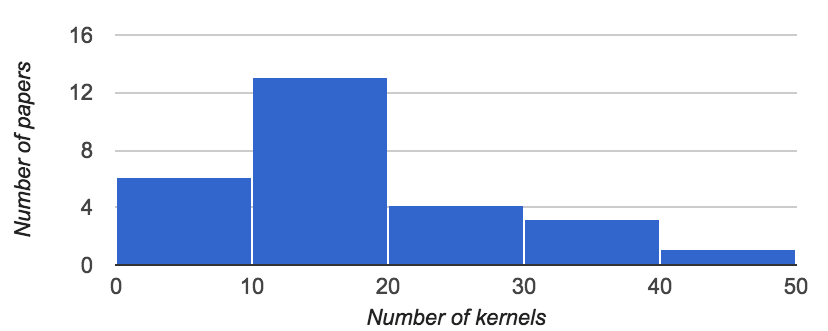
\includegraphics[width=\columnwidth]{img/benchmark-quantitiy-distribution}
%   % \begin{tikzpicture}
%   %   \tikzstyle{every node}=[font=\scriptsize]
%   %   \begin{axis}[
%   %     width=\columnwidth,
%   %     height=4cm,
%   %     ybar,
%   %     ymin=0,
%   %     xlabel={\#. benchmark kernels},
%   %     ylabel={\#. papers},
%   %     ],
%   %     \addplot +[
%   %     hist={
%   %       bins=5,
%   %       data min=0,
%   %       data max=50
%   %     }
%   %     ] table [y index=0] {data/benchmark-quantities.csv};
%   %   \end{axis}
%   % \end{tikzpicture}
%   \caption{%
%     Number of benchmark kernels used in GPGPU research papers. The
%     median value is 14.%
%   }
%   \label{fig:benchmark-quantity-distribution}
% \end{figure}

\begin{figure}%[t]
  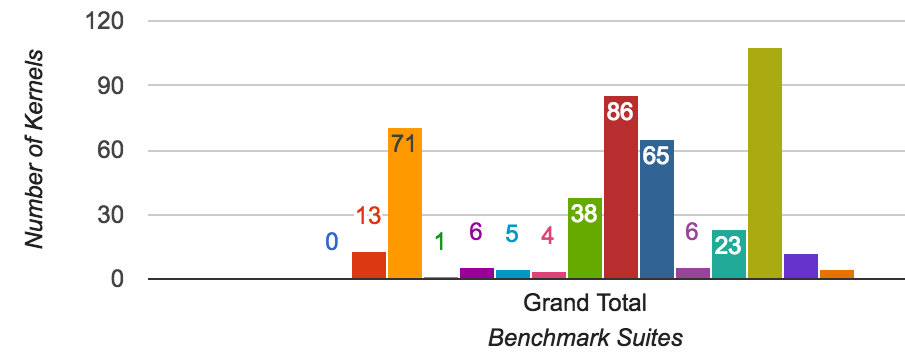
\includegraphics[width=\columnwidth]{img/benchmark-suite-distribution}
  \caption{%
    Origins of benchmark kernels used in GPGPU research papers. The 4
    most frequently used benchmark suites account for 74\% of all
    kernels used.%
  }
  \label{fig:benchmark-suite-distribution}
\end{figure}


\subsection{Motivation}\label{sec:motivation}

\begin{figure}%[t]
  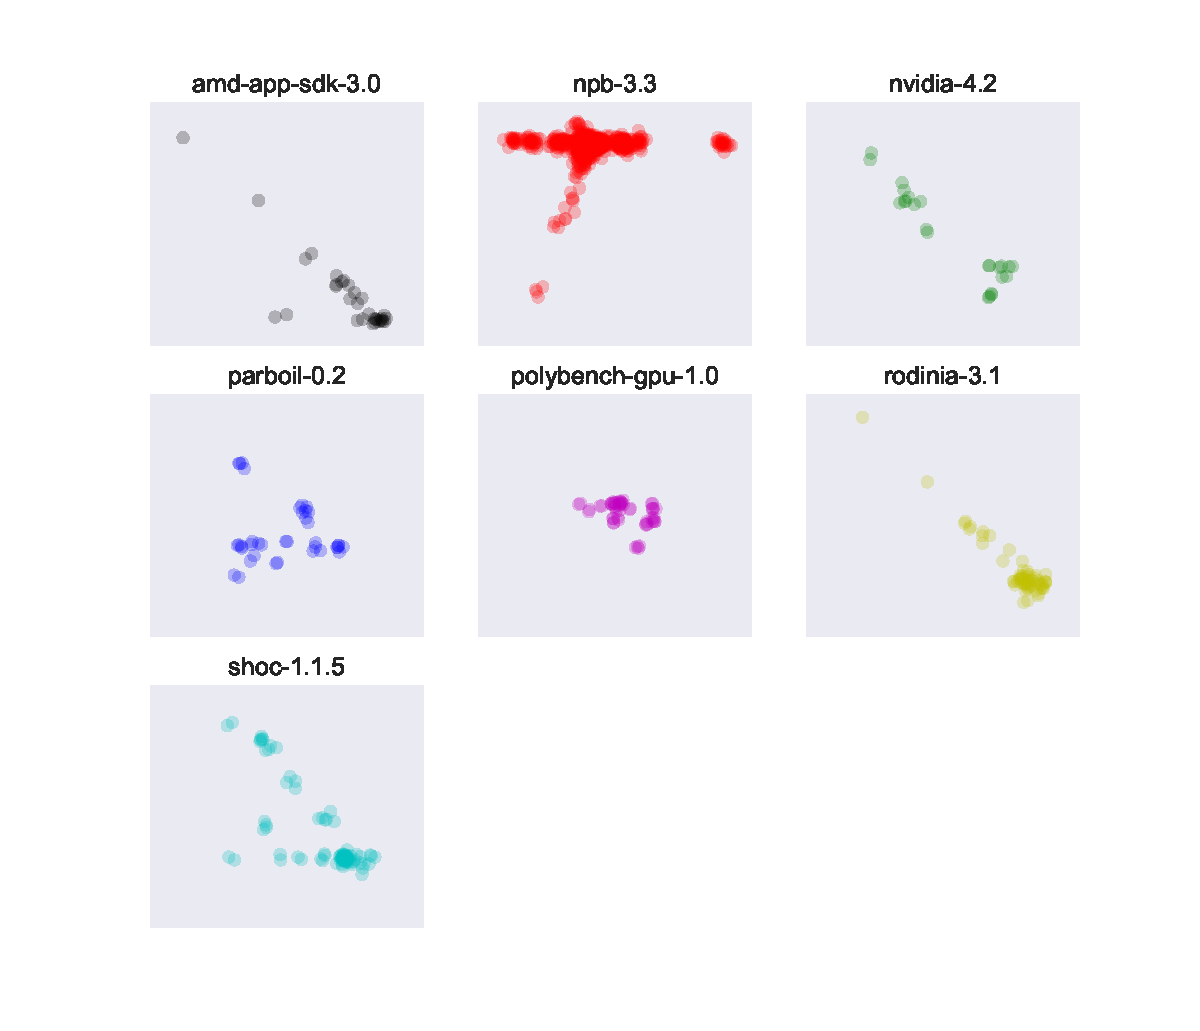
\includegraphics[width=\columnwidth]{img/pca-suites}
  \caption{%
    A two dimensional projection of the feature space of popular
    benchmarking suites.%
  }
  \label{fig:pca-benchmarks}
\end{figure}

TODO: state-of-the-art is laborious and error prone stochastic
template substitution, doesn't explore space.


\subsection{Contributions}

This paper makes the following contributions:%
\begin{itemize}
\item To the best of our knowledge, we are the first to apply machine
  learning over open source repositories in order to model the
  patterns of usage in a programming language.
\item Our novel system for synthesizing representative compute kernels
  using deep learning solves two issues for representative
  benchmarking: the limited quantity of benchmarks available, and the
  need to behavior that is representative of common use cases.
\item Experimental results show that the performance of a
  state-of-the-art autotuner is improved by XXX\% with the addition of
  benchmarks generated using our system.
\item Tool \textsc{CLgen} for generating OpenCL kernels using a deep
  learning network, and \textsc{CLdrive} for driving these generated
  kernels.
\end{itemize}


\section{Synthesizing Compute Kernels}\label{sec:synthesizing-compute-kenrels}

Overview of methodology. Figure~\ref{fig:structure}.

\paragraph{Assembling the Language Corpus} Mining GitHub, noisy
dataset.


\paragraph{Learning the Implementation Space} Program rewriting, LSTM,
character-level language model.


\paragraph{Synthesizing Compute Kernels} Sampling learned model using
function prototypes, rejection sampler, program checker.


\begin{figure*}%[t]
  \centering
  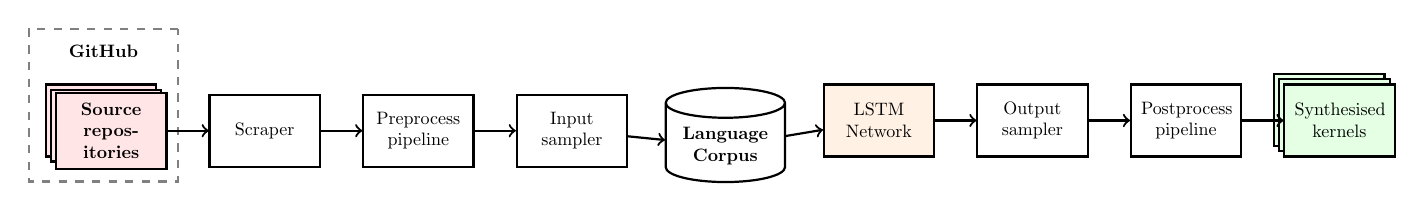
\begin{tikzpicture}[%
  auto,
  thick,
  scale=1,
  every node/.style={scale=0.65},
  node distance = 3cm,
  % Database shape:
  database/.style={%
    draw,
    cylinder,
    cylinder uses custom fill,
    shape border rotate=90,
    aspect=0.25
  }
  ]

  % Nodes:
  \node (t-start3) [block, fill=red!10, xshift=-.2cm, yshift=.2cm] {};
  \node (t-start2) [block, fill=red!10, xshift=-.1cm, yshift=.1cm] {};
  \node (t-start) [block, fill=red!10] {\textbf{Source repositories}};

  \node (t-scraper) [block, right of=t-start] {Scraper};
  \node (t-preprocess) [block, right of=t-scraper] {Preprocess pipeline};
  \node (t-input-sampler) [block, right of=t-preprocess] {Input sampler};
  \node (t-corpus) [database, right of=t-input-sampler, yshift=-.3cm] {\textbf{\begin{tabular}{c}Language\\Corpus\end{tabular}}};
  \node (t-network) [block, right of=t-corpus, fill=orange!10, yshift=.5cm] {LSTM Network};
  \node (t-output-sampler) [block, right of=t-network] {Output sampler};
  \node (t-postprocess) [block, right of=t-output-sampler] {Postprocess pipeline};
  \node (t-end3) [block, fill=green!10, right of=t-postprocess, xshift=-.2cm, yshift=.2cm] {};
  \node (t-end2) [block, fill=green!10, right of=t-postprocess, xshift=-.1cm, yshift=.1cm] {};
  \node (t-end) [block, fill=green!10, right of=t-postprocess] {Synthesised kernels};

  \node (github) [draw, dashed, color=gray, yshift=.5cm, xshift=-.15cm, inner ysep=1cm, inner xsep=.75cm, label={[yshift=-.7cm]\textbf{GitHub}}, fit=(t-start)] {};

  % Connectors:
  \draw[->] (t-start) -- (t-scraper);
  \draw[->] (t-scraper) -- (t-preprocess);
  \draw[->] (t-preprocess) -- (t-input-sampler);
  \draw[->] (t-input-sampler) -- (t-corpus);
  \draw[->] (t-corpus) -- (t-network);
  \draw[->] (t-network) -- (t-output-sampler);
  \draw[->] (t-output-sampler) -- (t-postprocess);
  \draw[->] (t-postprocess) -- (t-end);
\end{tikzpicture}

  \caption{%
    The kernel synthesis pipeline.%
  }
\label{fig:structure}
\end{figure*}


\section{Assembling Language Corpus}\label{sec:lang-corpus}

We collect a large code corpus from
GitHub\footnote{\url{https://github.com/}}. This took one day on a
single machine.

Rejection sampling to remove noise from dataset. Check that compiles.

Alternative source of data: \emph{GHTorrent}~\cite{Gousios2014a}.

Minimizing non-functional variance using clang libraries and tools:
\begin{itemize}
\item Pre-process source to remove macros and conditional
  compilation.
\item Loss-less vocabulary size reduction with AST rewriting of
  identifiers.
\item Automatically enforcing code style with formatting tools.
\end{itemize}

Pre-processing pipeline: Implemented on
LLVM\footnote{\url{http://llvm.org/}},
clang%\footnote{\url{http://clang.llvm.org/}}
, and libclc%\footnote{\url{http://libclc.llvm.org/}}
.

\begin{figure}%[t]
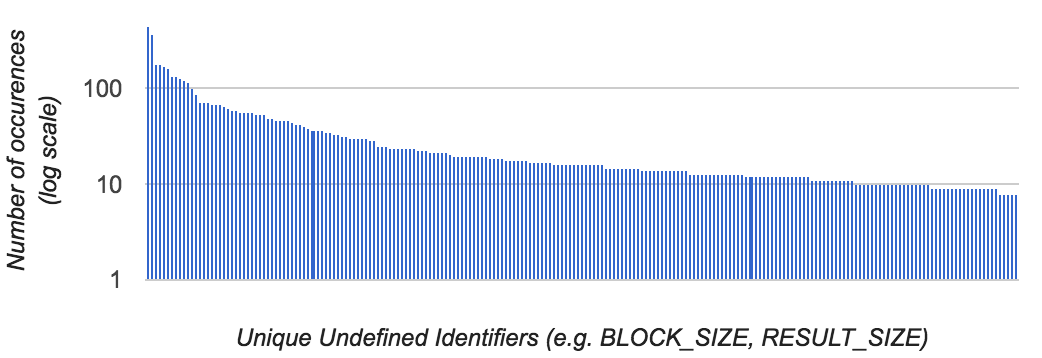
\includegraphics[width=\columnwidth]{img/undeclared-identifiers.png}
\caption{%
  Undeclared identifier occurrences in OpenCL sources.
  % all 1023 unique identifiers in the OpenCL source codes set. The most
  % frequently used undeclared identifier is \texttt{LOCAL\_SIZE\_LIMIT}
  % (462 occurrences). The 60 most used identifiers account for 50\% of
  % errors.%
}
\end{figure}

Compile to LLVM byte code using libclc. Through analyzing 148k lines of
compilation errors, we created a shim header to include common missing
things. Include shim header which adds inferred values for common
typedefs (e.g. FLOAT\_T to float), and best guesses for common
constants (e.g. WGSIZE). Listing~\ref{lst:shim}

Preprocessor is a unique challenge to C family of languages. Shim
decreases the discard rate from 40\% to 32\% (responsible for an
additional 88k lines of code in the language corpus). These macros may
be harmlessly redefined within files.

\lstset{language=C}
\begin{lstlisting}[%
  float,%
  caption=The shim header file.
]
/* Enable OpenCL features */
#define cl_clang_storage_class_specifiers
#define cl_khr_fp64
#include <clc/clc.h>

/* Inferred types */
typedef float FLOAT_T;
typedef unsigned int INDEX_TYPE;|\Suppressnumber|
... (36 more)|\Reactivatenumber|

/* Inferred constants */
#define M_PI 3.14025
#define WG_SIZE 128|\Suppressnumber|
... (185 more)|\Reactivatenumber|
\end{lstlisting}

\section{Learning the Implementation Space}\label{sec:ml}

% \subsection{Machine Learning Model}

We use the Long Short-Term Memory (LSTM) architecture of Recurrent
Neural Network~\cite{Hochreiter1997,Mikolov2015}. LSTMs are proving to
be a powerful learning tool with applications from speech recognition
to image captioning. LSTMs for language
modeling~\cite{Sundermeyer2012}. No features. LSTM
implementation\footnote{\url{https://github.com/jcjohnson/torch-rnn}}.

%
% $ python scripts/preprocess.py --input_txt data/github.txt --output_h5 data/deleteme.h5 --output_json data/deleteme.json
% Total vocabulary size: 94  # input_size
% Total tokens in file: 33057927  # 33 million tokens
%  Training size: 26446343  # training / validation / test split
%  Val size: 3305792
%  Test size: 3305792
% Using dtype  <type 'numpy.uint8'>
%
% FIXME: Verify the input size and re-compute # parameters:
% http://stackoverflow.com/questions/38080035/how-to-calculate-the-number-of-parameters-of-an-lstm-network
%
% params = 4 * ((size_of_input + 1) * size_of_output + size_of_output^2)
%
%   size_of_input = 94
%   size_of_output = 2048
We used a 3 layer LSTM model of 2048 nodes each for a total of 17
million parameters. We trained the model using stochastic gradient
descent for 50 epochs, using an initial learning rate of 0.002 and
decaying by a factor of a half every 5 epochs. Training took two weeks
on a single machine using an Nvidia GTX Titan.

% Vocabulary size 96. Training size 33 million tokens. Learned model
% 648 MB.


\section{Synthesizing Compute Kernels}\label{sec:syn}

\lstset{language=[OpenCL]C}
\begin{lstlisting}[%
  float,%
  numbers=left,
  caption=Compute kernels generated by our network.
]
__kernel void A(__global float* a,
                __global float* b,
                __global float* c,
                const int d) {
    int e = get_global_id(0);

    if (e < d)
        b[e] = a[e] + 0xb5ca050f;
    barrier(1);

    if (e < d) {
        e = a[e];
        c[e] = a[e];
    }
    barrier(1);

    for (int e = 0; e < get_global_id(0); e++) {
        if (a[e] < a[e] || c == 1) {
            c[e % 16] = 0;
        }
    }
}|\Suppressnumber|
|\Reactivatenumber|
__kernel void A(__global float* a,
                __global float* b,
                const int c) {
    int d = get_global_id(0);
    a[d] = (b[d] < a[d]) ? 63 : d * 8 + c * 32;
}|\Suppressnumber|
|\Reactivatenumber|
__kernel void A(__global float* a,
                __global float* b,
                __global float* c,
                const int d) {
    int e = get_global_id(0);
    if (e < d) {
        c[e] = a[e] + b[e];
    }
    barrier(2);

    if (e >= d)
        c[e] = b[e] + c[e - 1];

    if (e < 0)
        b[e] = a[e] + a[e - 1];
    if (0 <= c)
        c[e] = a[e] + 1;
    else
        b[e] = b[e] + 2;

    barrier(1);

    if (e < d) {
        a[e] = a[e];
    }
}
\end{lstlisting}

% \begin{figure}%lst:ex
%   \lstset{language=[OpenCL]C}
%   \centering
%   \subfloat[][]{%
%     \lstinputlisting[frame=single]{lst/ex1.cl}%
%   }\\
%   \subfloat[][]{%
%     \lstinputlisting[frame=single]{lst/ex2.cl}%
%   }\\
%   \subfloat[][]{%
%     \lstinputlisting[frame=single]{lst/ex3.cl}%
%   }
%   \caption{%
%     Compute kernels generated by our network.%
%   }
%   \label{lst:ex}
% \end{figure}

Given a function prototype.

Sample kernels with balanced brackets.

Rejection sampler (same as preprocess pipeline).

Undefined behavior.

Examples of kernels generated by our model for a given
prototype. Figure~\ref{lst:ex}.


\paragraph{Driving Synthesized kernels}

The method for determining whether a kernel is interesting or not is:

\begin{itemize}
\item Create 4 equal size payloads $A_1$, $B_1$, $A_2$, $B_2$.
  Restrictions: $A_1=A_2$, $B_1=B_2$, $A_1 \ne B_1$, $A_1 =$“known
  values” (i.e. $\left[0, 1, 2 \ldots n\right]$). $B_1=$random values.
\item Run kernel $k$ 4 times: $k(A_{1in}) \rightarrow A_{1out}$,
  $k(B_{1in}) \rightarrow B_{1out}$,
  $k(A_{2in}) \rightarrow A_{2out}$,
  $k(B_{2in}) \rightarrow B_{2out}$.
\item Assert: $A_{1out}=A_{2out}$, $B_{1out}=B_{2out}$,
  $A_{1out} \ne B_{1out}$.
\end{itemize}

Outcomes: \texttt{E\_BAD\_CODE} program doesn’t compile;
\texttt{E\_BAD\_ARGS} driver failed to create payload;
\texttt{E\_TIMEOUT} execution took longer than $T$ seconds;
\texttt{E\_OUTPUTS\_UNCHANGED} $X_{out}=X_{in}$ code either does nothing, or
doesn’t write result; \texttt{E\_INPUT\_INSENSITIVE} $X_{out}=Y_{out}$ code
does the same thing irrespective of input;
\texttt{E\_NONDETERMINISTIC} $X_{1out}=X_{2out}$ code has non-deterministic
behavior.


TODO: Post-process, if ratio of CI to mean exceeds threshold.


\section{Experimental Methodology}\label{sec:methodology}

To evaluate the effectiveness we apply to a state-of-the-art autotuner
for OpenCL kernels.

\subsection{Experimental Setup}\label{subsec:experimental-setup}

\paragraph{Predictive Model} We reproduce the predictive model from
\citeauthor{Grewe2013}~\cite{Grewe2013}. Decision Tree classifier
implemented in Python~\cite{Pedregosa2012}. Features from static
source code and dynamic runtime information, summarized in
Table~\ref{tab:cgo13-features}.

\begin{table}% tab:cgo13-features
  \scriptsize
  \centering
  \begin{tabular}{l L{4.5cm}}
    \toprule
    \multicolumn{2}{c}{\textbf{Combined Code Features}} \\
    \midrule
    \texttt{F1: transfer/(comp+mem)} & commun.-computation ratio \\
    \texttt{F2: coalesced/mem} & \% coalesced memory accesses \\
    \texttt{F3: (localmem/mem)$\times$wgsize} & ratio local to global mem accesses $\times$\\
                            & \# work-items \\
    \texttt{F4: comp/mem} & computation-mem ratio\\
    \bottomrule
  \end{tabular}
  \caption{%
    List of code features.
  }
  \label{tab:cgo13-features}
\end{table}


\paragraph{Benchmarks}

% Generate using:
%
% cd ~/phd/lab/smith/benchmarks/ && ./list-benchmarks data/training-combined.csv
\begin{table}% tab:benchmarks
  \scriptsize
  \centering
  \begin{tabular}{l r r r}
    \toprule
    & \textbf{Version} & \textbf{\#. programs} & \textbf{\#. kernels}\\
    % TODO: \#. datasets
    \midrule
    \textbf{NPB (SNU~\cite{Seo2011})} & 1.0.3 & 7 & 114 \\
    \textbf{Rodinia~\cite{Che2009}} & 3.1 & 14 & 31 \\
    \textbf{NVIDIA SDK} & 4.2 & 6 & 12 \\
    \textbf{AMD SDK} & 3.0 & 12 & 16 \\
    \textbf{Parboil~\cite{Stratton2012}} & 0.2 & 6 & 8 \\
    \textbf{PolyBench~\cite{Grauer-Gray2012}} & 1.0 & 14 & 27 \\
    \textbf{SHOC~\cite{Danalis2010}} & 1.1.5 & 12 & 48 \\
    \textbf{Synthetic} & - & - & TODO \\
    \bottomrule
  \end{tabular}
  \caption{%
    List of benchmark suites.
  }
  \label{tab:benchmarks}
\end{table}

Table~\ref{tab:benchmarks}. Notes: Parboil: opencl\_base
implementation. Ignored benchmarks from the SDKs which were
inappropriate (e.g. testing multi-GPU support, or some
platform-specific extension).

Rewrote typedefs.

Limitation of system: can't use synthesize kernels with struct
arguments. Ignored kernels with struct args: %
parboil-bfs, %
parboil-mri-q, %
rodinia-b-tree, %
rodinia-dwt2d, %
rodinia-heartwall, %
rodinia-lavamd, %
rodinia nearest neighbor.


\paragraph{Platforms} We evaluate our approach on two 64-bit CPU-GPU
systems, detailed in Table~\ref{tab:platforms}. Platform A uses
OpenSUSE 12.3 and GCC 4.7.2; Platform B uses Ubuntu 14.04 and GCC
x. The AMD implementation of OpenCL 1.2 is used for both.

\begin{table}% tab:platforms
  \scriptsize
  \centering
  \begin{tabular}{l l l l}
    \toprule
    %         monza CPU            monza GPU          diana GPU
    & \textbf{Intel CPU} & \textbf{AMD GPU} & \textbf{NVIDIA GPU} \\
    \midrule
    \textbf{Model} & Core i7-3820 & Tahiti 7970 & GTX 970 \\
    \textbf{Frequency} & 3.6 GHz & 1000 MHz & 1050 MHz \\
    \textbf{\#. Cores} & 4 & 2048 & 1664 \\
    \textbf{Memory} & 8 GB & 3 GB & 4 GB \\
    \textbf{Throughput} & 105 GFLOPS & 3.79 TFLOPS & 3.90 TFLOPS \\
    \textbf{Driver} & AMD 1526.3 & AMD 1526.3 & NVIDIA 361.42 \\
    \textbf{Compiler} & GCC 4.7.2 & GCC 4.7.2 & GCC 5.4.0 \\
    \bottomrule
  \end{tabular}
  \caption{Experimental platforms.}
  \label{tab:platforms}
\end{table}


\paragraph{Datasets}


\subsection{Methodology}

Followed the methodology of~\cite{Grewe2013}.

Statistical soundness.

Leave-one-out cross validation.


\section{Experimental Results}\label{sec:results}

Median num samples per kernel. Ratio 95\% CI / mean.

\subsection{Comparison with state-of-the-art}

Autotuner can't learn across benchmark
suite. Table~\ref{tab:bench-xval-bench}.

\begin{table}%[t]
  \centering
  \subfloat[][Platform A]{%
    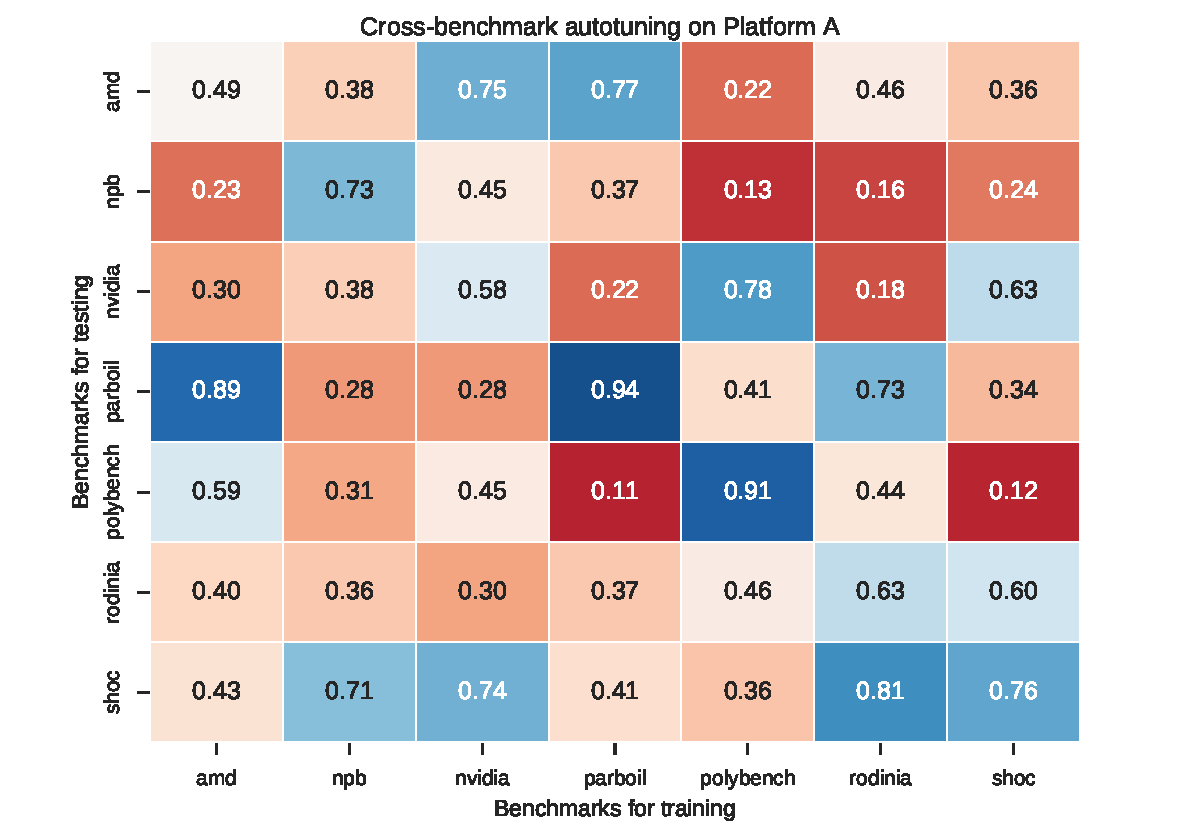
\includegraphics[width=\columnwidth]{img/bench-xval-bench-A}%
    \label{tab:bench-xval-bench-a}}\\
  \subfloat[][Platform B]{%
    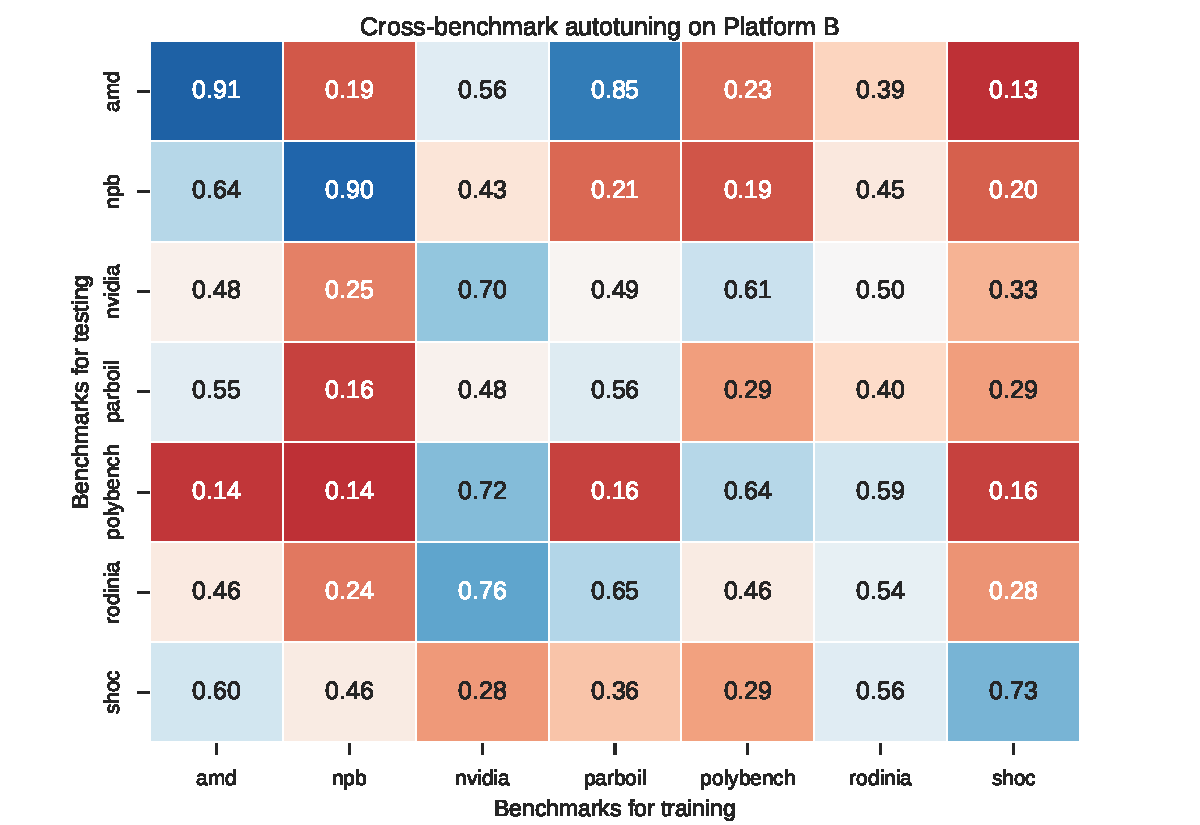
\includegraphics[width=\columnwidth]{img/bench-xval-bench-B}%
    \label{tab:bench-xval-bench-b}}
  \caption{%
    Cross-benchmark autotuning results.}
\label{tab:bench-xval-bench}
\end{table}

\subsection{Generated Compute Kernels}\label{subsec:compute-kernels}

Evaluating \emph{RQ1}. What's the ratio of ``good'' code? How long did
it take to sample?

Ratio of generated kernels rejected by postprocess pipeline:
%  echo "100 - $(smith-explore synthetic.db | grep "Number of good preprocessed" | cut -d'(' -f2 | cut -d'%' -f1)" | bc -l | xargs printf '%d\\%%'
93\%. Ratio of postprocessed kernels which do not pass cldrive
conformance test:
% TODO: command to generate this.
47\%. Total ratio of ``good'' kernels: 3\%.

Two days sampling on a single machine. TODO: Estimate bytes / second
of generated ``good'' kernels.

TODO: Plot distribution of static features from benchmark suites,
GitHub, and generated synthesis.

TODO: Table of cldrive rejection categories.

Comparing feature space of benchmarks and generated
kernels. Figure~\ref{fig:bench-eigens}.

\begin{figure}%[t]
  % Generated with:
  %
  % smith-plot eigens ~/phd/lab/smith/benchmarks/data/training-combined.csv --group suite -o ~/phd/docs/wip-smith/img/bench-eigens.pdf --width 7 --height 7
  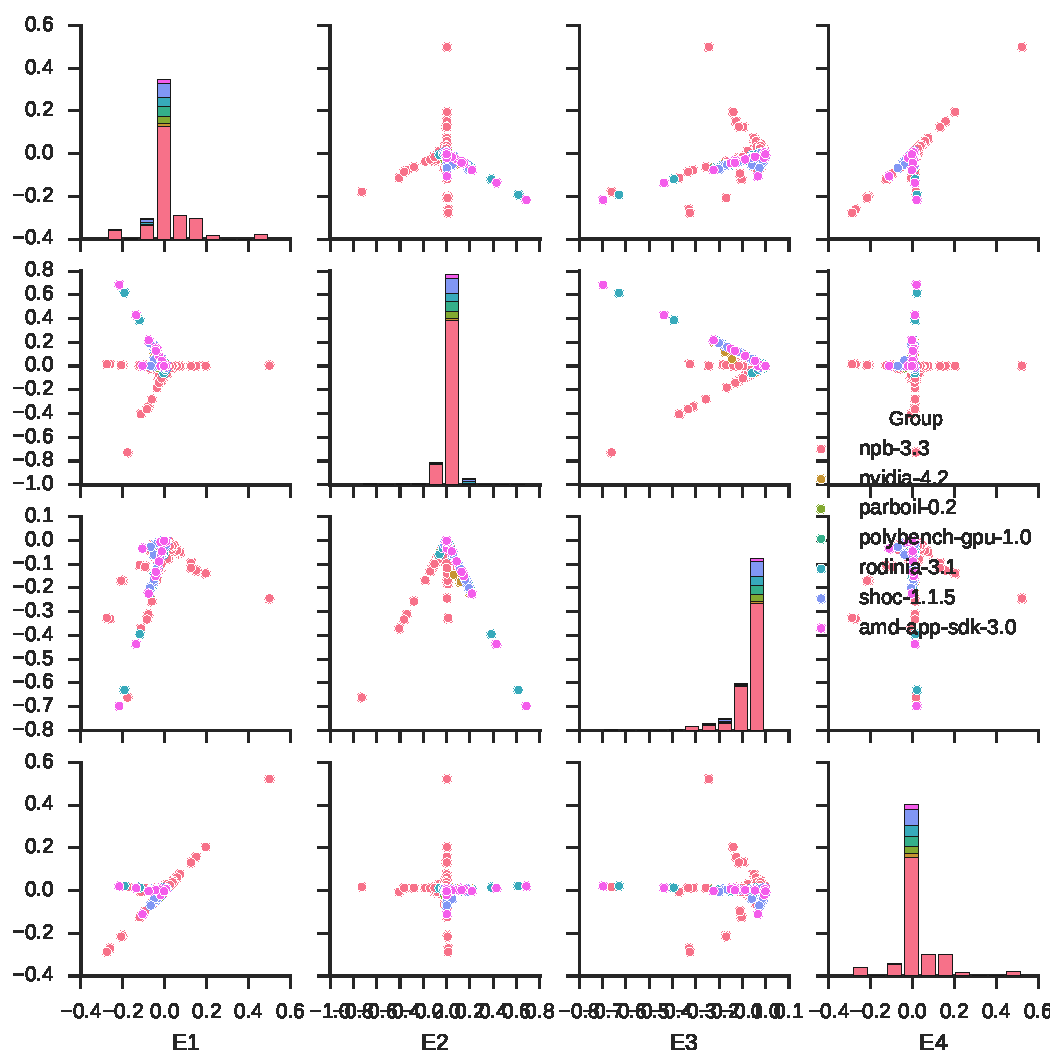
\includegraphics[width=\columnwidth]{img/bench-eigens}%
  \caption{%
    Eigenspace of benchmark applications.%
  }
  \label{fig:bench-eigens}
\end{figure}


\subsection{Qualitatively Evaluating Generated Code}\label{subsec:}

20 OpenCL developers, each shown 10 samples of code. For each sample,
50\% chance of being generated by our network, and 50\% chance of
either GitHub mined or benchmark kernel. Related works which have used
Non-Interactive Turing Tests~\cite{Gao2015a,Zhang2016}.


\subsection{Predicting Execution Device}\label{subsec:predictive-model}

Evaluating \emph{RQ2}. Classification accuracy and speedups. Compare
prediction performance with and without additional synthetic
benchmarks.

\begin{figure}
  \centering
  \subfloat[][AMD]{%
    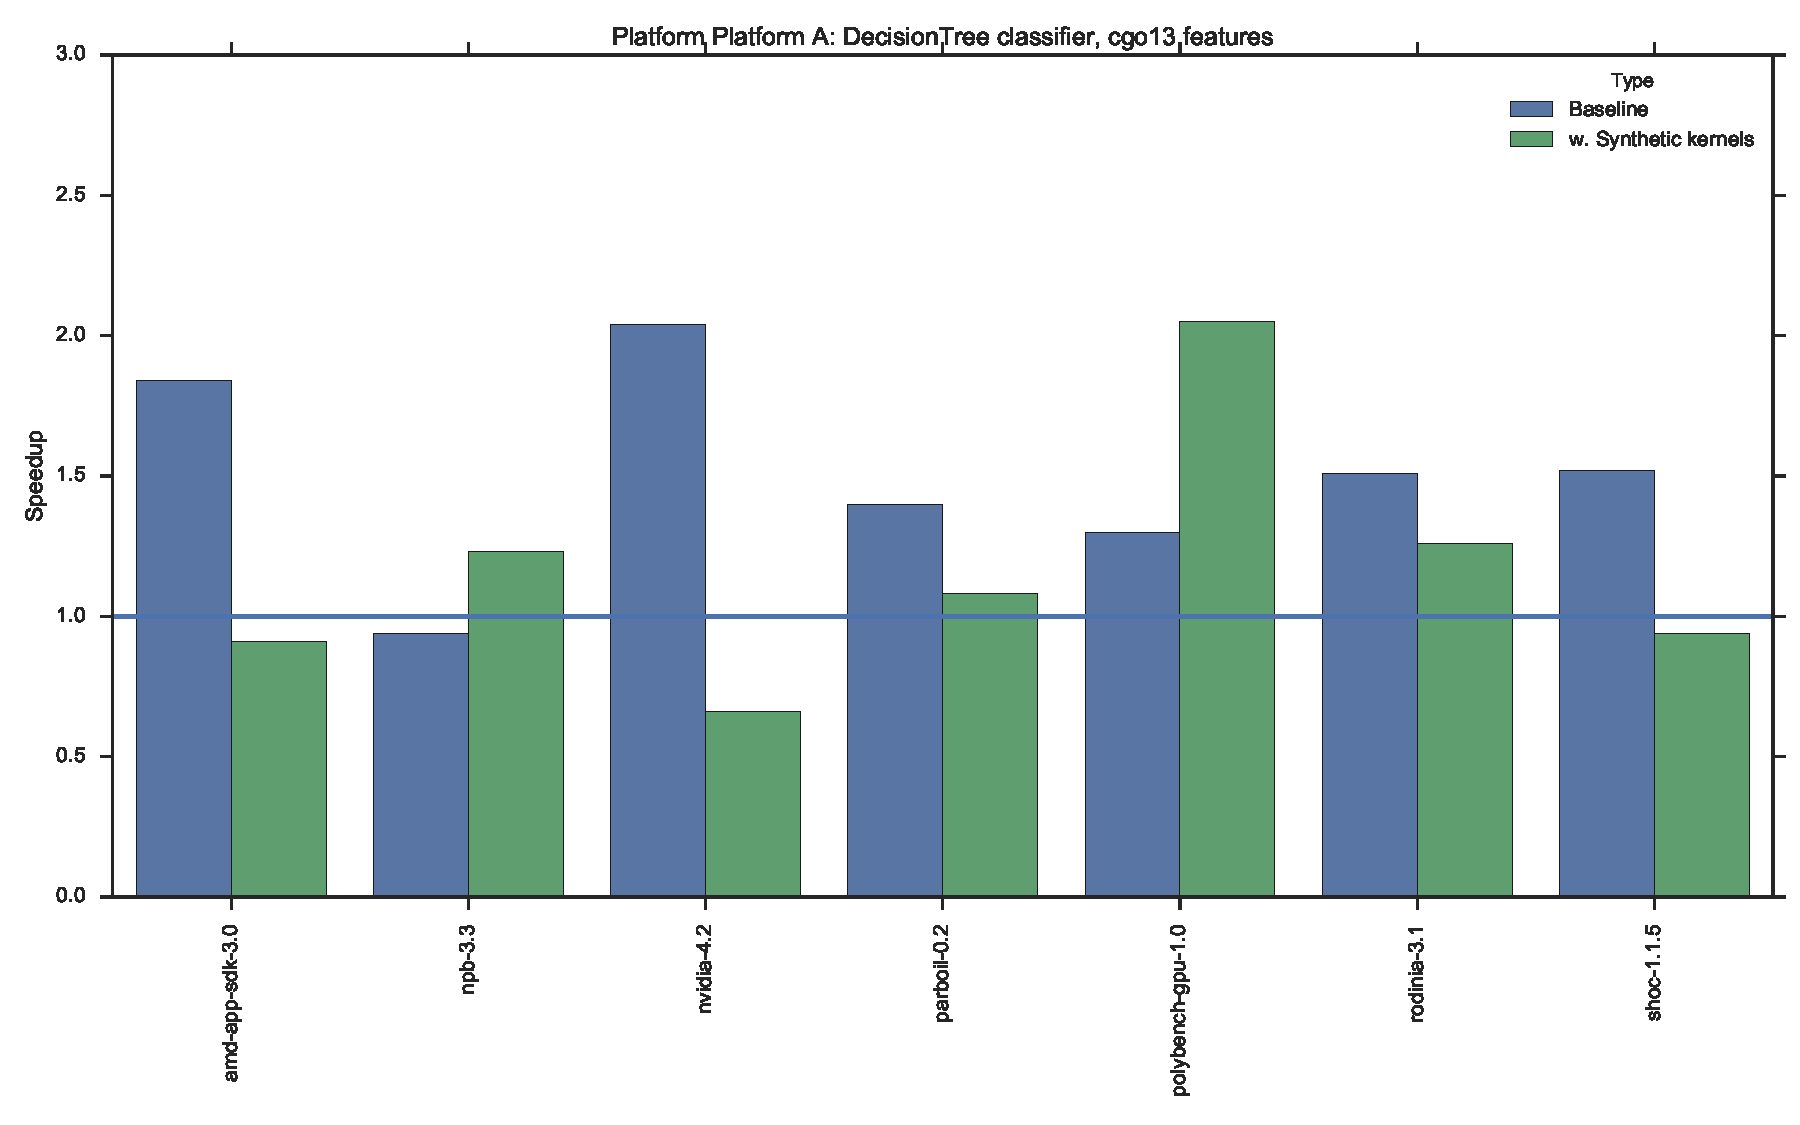
\includegraphics[width=\columnwidth]{img/npb-amd}%
    \label{fig:npb-amd}}\\
  \subfloat[][NVIDIA]{%
    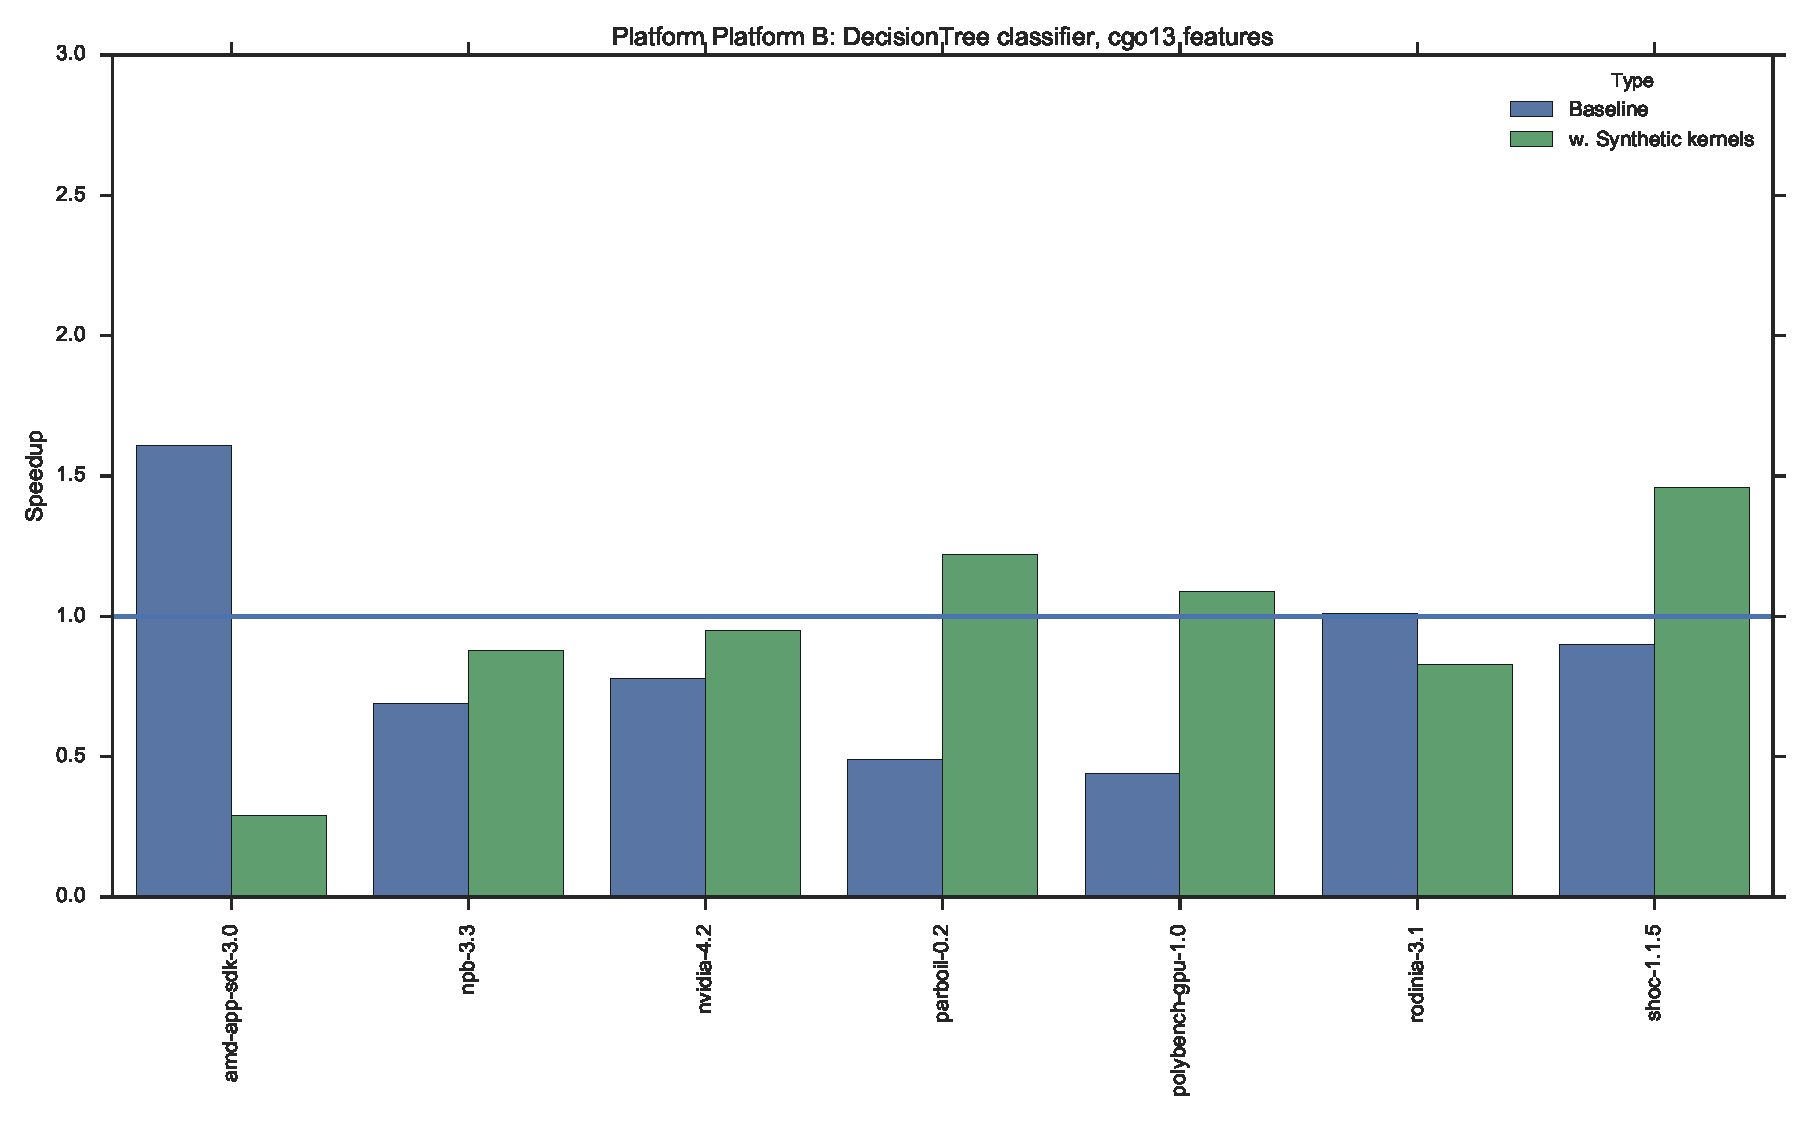
\includegraphics[width=\columnwidth]{img/npb-nvidia}%
    \label{fig:npb-nvidia}}
  \caption{%
    Comparison of prediction performance with and without synthetic
    kernels on \protect\subref{fig:npb-amd}~AMD and
    \protect\subref{fig:npb-nvidia}~NVIDIA.%
  }
\label{fig:npb}
\end{figure}

\begin{figure}
  \centering
  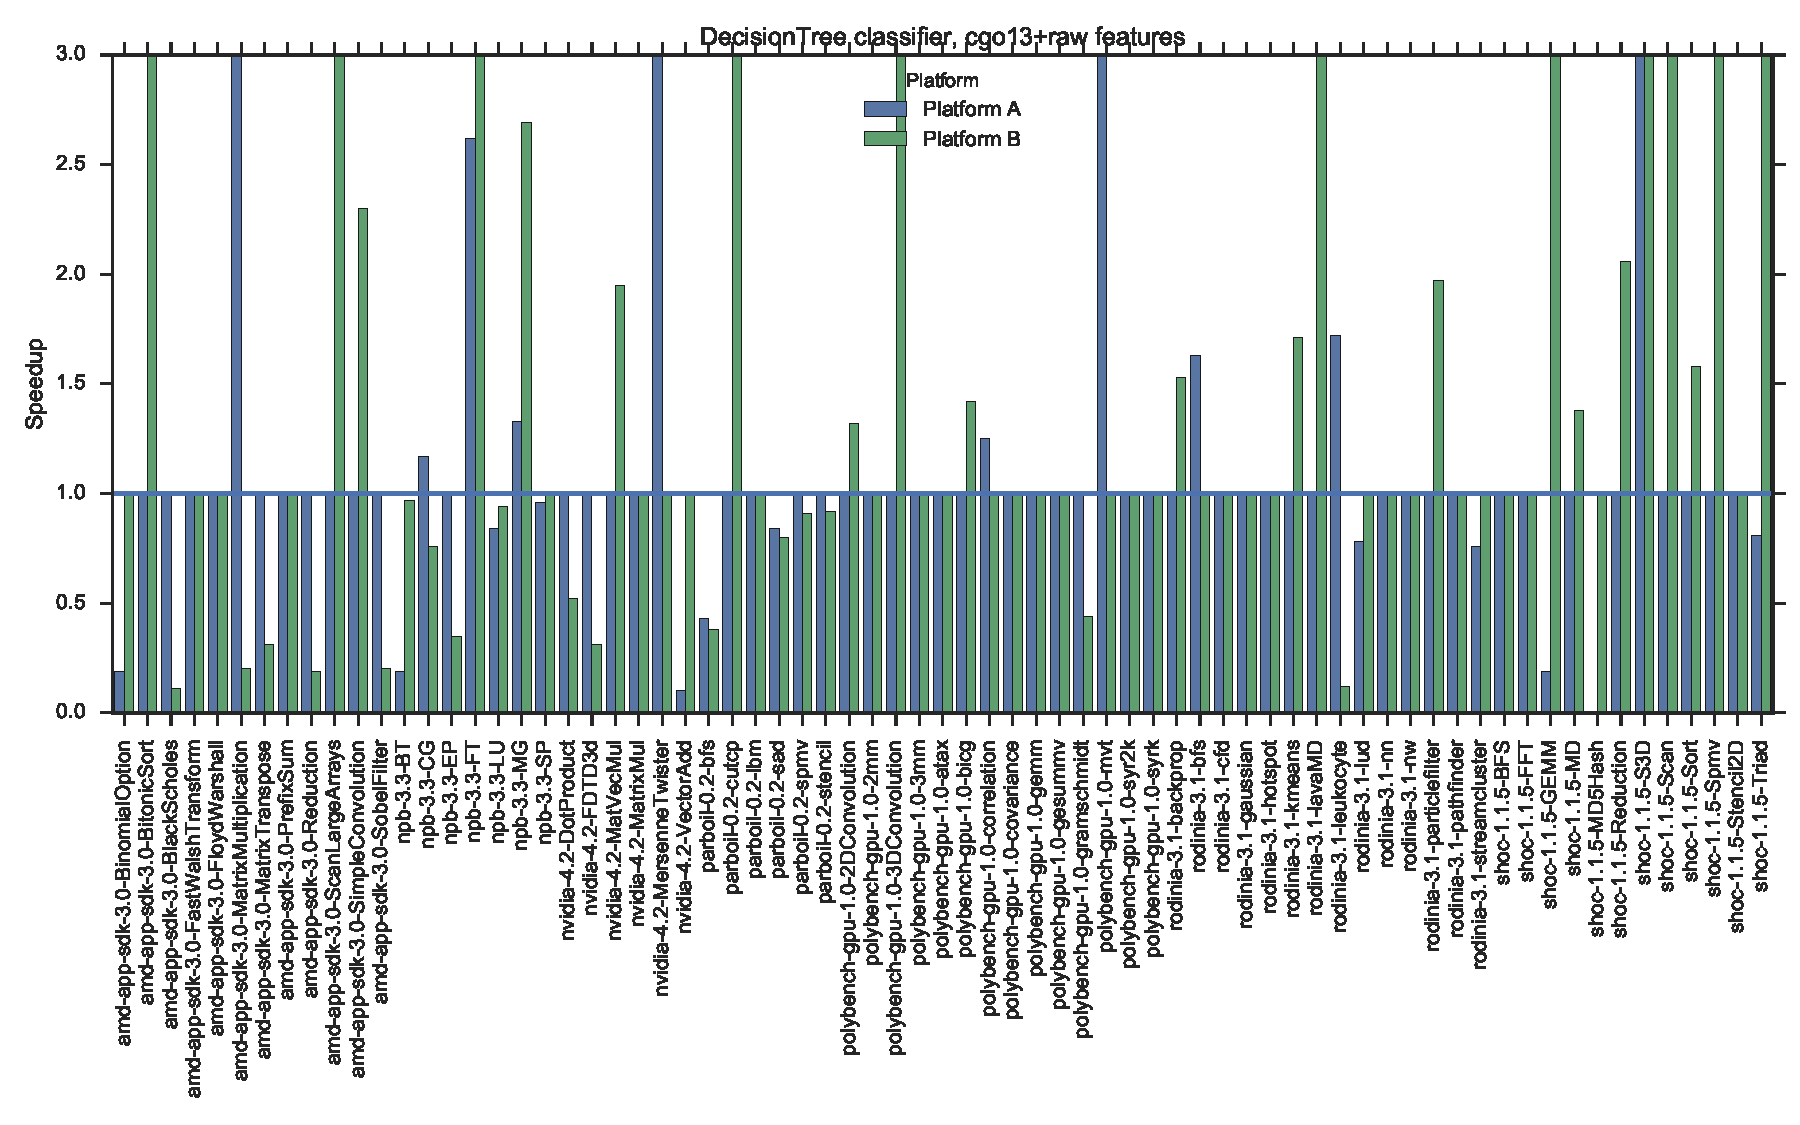
\includegraphics[width=\columnwidth]{img/xval-benchmarks}%
  \caption{%
    Speedups of predictions using extended autotuner trained with
    synthetic benchmarks over hand-selected benchmarks.%
  }
\label{fig:xval-benchmarks}
\end{figure}

\begin{figure}%[t]
  \subfloat[][]{%
    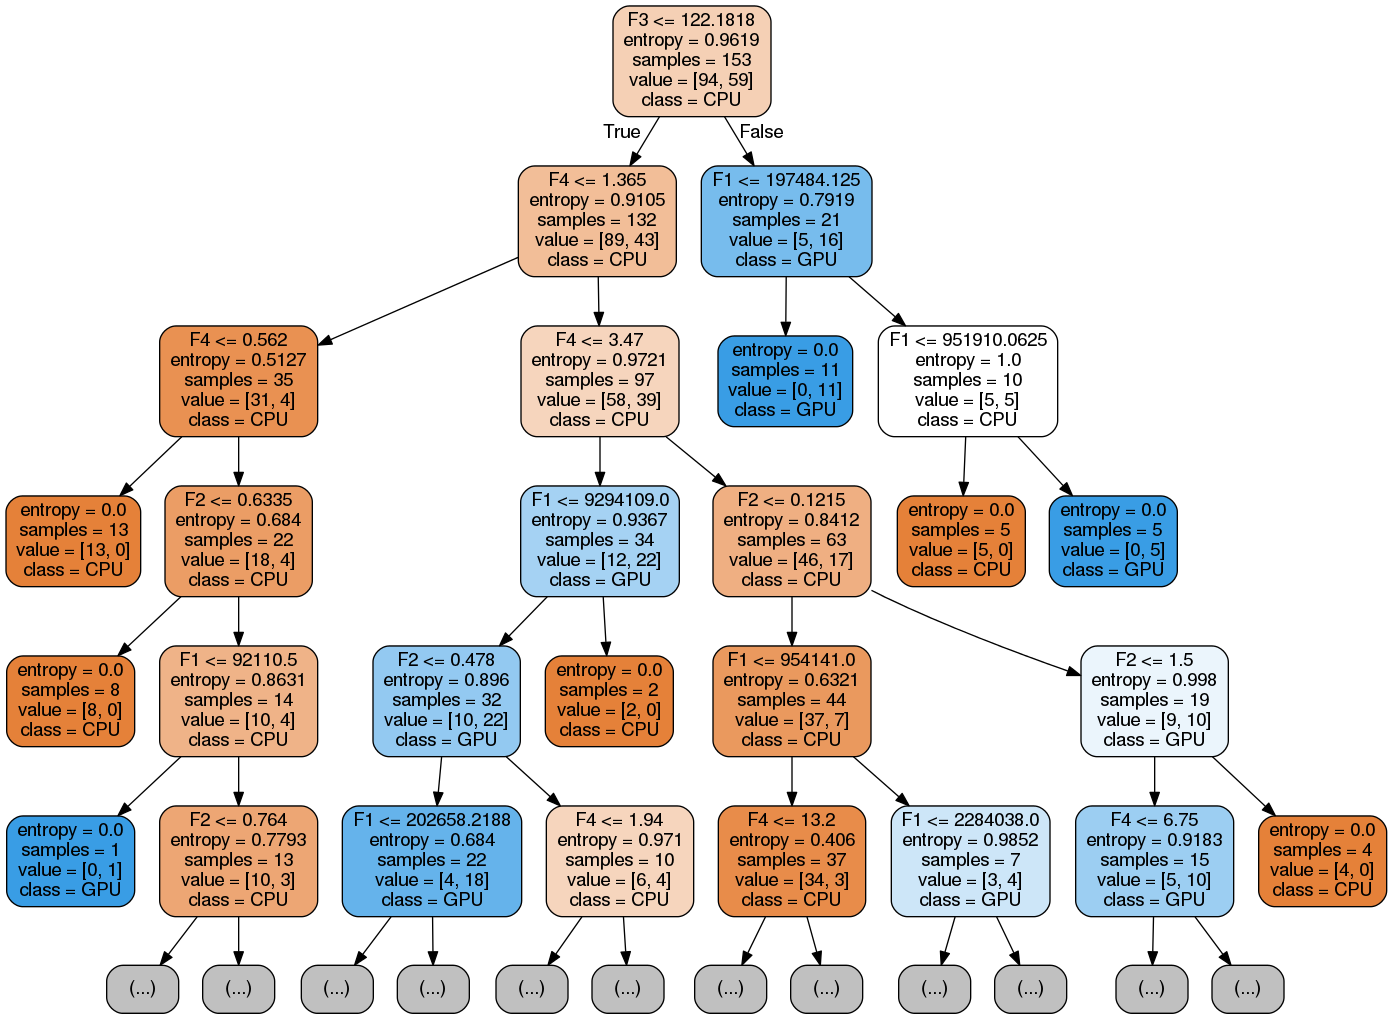
\includegraphics[width=\columnwidth]{img/tree}\label{fig:tree-a}%
  }\\
  \subfloat[][]{%
    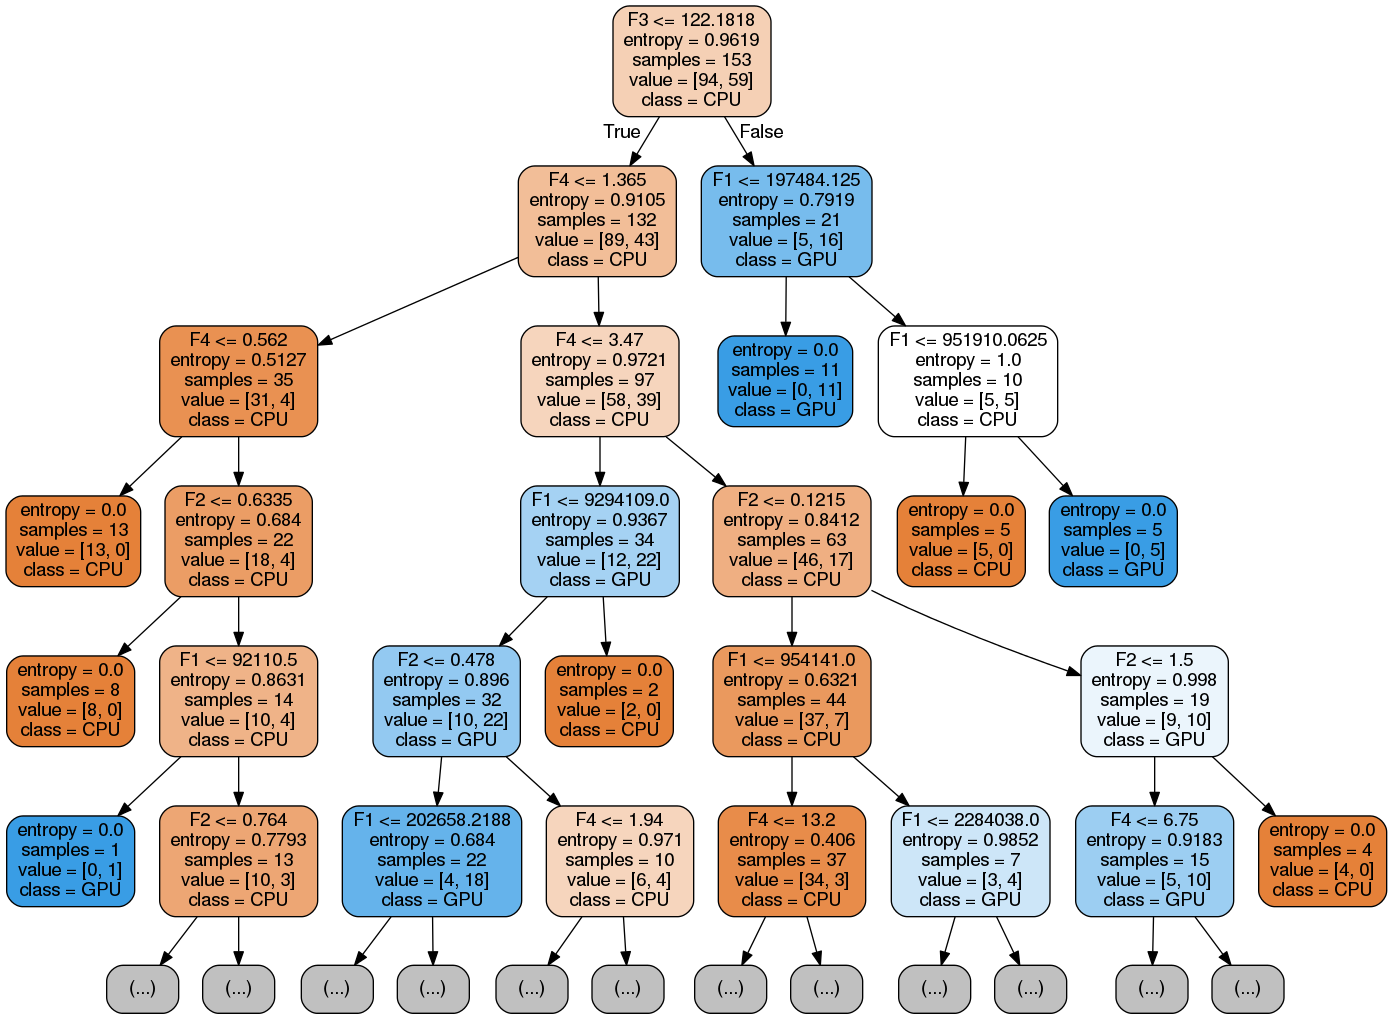
\includegraphics[width=\columnwidth]{img/tree}\label{fig:tree-b}%
  }
  \caption{%
    The model used for XXX on XXX, \protect\subref{fig:tree-a}~with and
    \protect\subref{fig:tree-b}~without synthetic kernels.%
  }
  \label{fig:trees}
\end{figure}


\section{Related Work}\label{sec:related-work}

Are benchmarks suites representative? Exploring the full performance
spectrum~\cite{Ryoo2015}. Characterizing workloads of Rodinia and
Parsec~\cite{Che2010}.

In previous work we used stochastic template substitution to generate
stencil benchmarks for autotuning~\cite{Cummins2015a}. This template
based approach is not general purpose, requires laborious human
effort, and does not guarantee to generate representative benchmarks.

Misc: Verifying GPU kernels~\cite{Betts2012}. Simulating OpenCL
kernels~\cite{Price2015}.

Machine Learning-based Performance Tuning:~\cite{Wen2015},
\cite{Magni2014}, \cite{Falch2015}. Domain specific:
Stencils~\cite{Garvey2015b}, \cite{Cummins2015a}. Input sensitive
autotuning~\cite{Ding2015}. Benchmark reduction~\cite{Castro2014}.


\paragraph{Representative Benchmarking} Designing
workloads~\cite{Eeckhout2002}. Characterization of NAS
OpenCL~\cite{Seo2011}. Characterization of
Rodinia~\cite{Che2010,Ryoo2015}. Analytic modeling to reduce
benchmarking costs~\cite{Kalibera2013}.


\paragraph{Program Generation} Template-based:
GENESIS~\cite{Chiu2015}.  Grammar-based: Csmith~\cite{Yang2012},
CLsmith~\cite{Pflanzer2016}. Mutation-based: JVM
fuzzing~\cite{Chena}. Goal-oriented: Generating linear
transforms~\cite{Voronenko2009}, synthesizing MapReduce
programs~\cite{Smith}, generating data structure
implementations~\cite{Loncaric2016}.


\paragraph{Mining Source Codes} Neural Networks for representing
programs~\cite{Bunel}.

Promises and perils of mining GitHub~\cite{Bird2009}.

Mining source code repositories at large
scale~\cite{Allamanis2013a,White2015a}. Machine learning for analyzing
code~\cite{Allamanis2014a,Raychev}. Aiding software
engineering~\cite{Allamanis2014,Bird2015}.

Previous studies have involved data mining of GitHub for analysis of
software engineering
practices~\cite{Wu2014,Guzman2014,Baishakhi2014a,Vasilescu2015}.


\paragraph{Deep Learning} This is the first application of deep
learning for synthesizing programs.

Deep Learning has been successful for synthesizing graphics
textures~\cite{Gatys2015a}, image captions~\cite{Vinyals}, colors for
black and white photographs~\cite{Zhang2016}, and artistic
style~\cite{Gatys2015}. DRAW: A Recurrent Neural Network For Image
Generation~\cite{Gregor2014}.


DeepAPI learns API usage from annotated snippets from
GitHub~\cite{Zhang2015a}.


\section{Conclusion}\label{sec:conclusion}

Addressing limitations of current approach: more data (we're mining
directly from GitHub so we're pretty close to the upper limit
already), improvements to the model (more parameters - overfitting,
switch to a token based vocabulary).

Future work: probabilistic grammar.


\acks

This work was supported by the UK Engineering and Physical Sciences
Research Council under grants EP/L01503X/1 (CDT in Pervasive
Parallelism), EP/H044752/1 (ALEA), and EP/M015793/1 (DIVIDEND).
% TODO: Zheng's acks

\label{bibliography}
\printbibliography


\end{document}
